 
 

\documentclass[french]{article}
\usepackage[T1]{fontenc}
\usepackage[utf8]{inputenc}
\usepackage{lmodern}
\usepackage[a4paper]{geometry}
\usepackage{babel}
\usepackage{subcaption}
\usepackage{graphicx}
\usepackage[nottoc,numbib]{tocbibind}
\usepackage{pdfpages}
\usepackage[hidelinks]{hyperref}
\usepackage{fullpage}
\usepackage{subfiles}

\usepackage{algorithm}
\usepackage{algorithmic}
\usepackage{minted}

\setminted{linenos}


\usepackage{amsthm}
\usepackage{amssymb}
\usepackage{amsmath}
\usepackage{bbold}
\theoremstyle{plain}
\newtheorem{thm}{Theorem}
\newtheorem{prop}{Proposition}
\newtheorem{coro}{Corollary}
\newtheorem{lem}{Lemma}

\theoremstyle{definition}
\newtheorem{defn}{Définition}
\newtheorem{exemple}{Example}


\theoremstyle{remark}
\newtheorem{rem}{Remark}
\newtheorem{exercice}{Exercize}
\newtheorem{quest}{Question}

%% Ensemble usuels 

\newcommand{\rel}{\mathbb{Z}}
\newcommand{\nat}{\mathbb{N}}
\newcommand{\rat}{\mathbb{Q}}
\newcommand{\real}{\mathbb{R}}
\newcommand{\complex}{\mathbb{C}}

\newcommand{\Esp}{\mathbb{E}}

\newcommand{\Z}{\rel}
\newcommand{\N}{\nat}
\newcommand{\Q}{\rat}
\newcommand{\R}{\real}
%\newcommand{\C}{\complex}
\newcommand{\ZZ}[1]{\relmod{#1}}

\newcommand{\unit}{\mathbb{U}}
\newcommand{\relmod}[1]{\rel/#1\rel}
\newcommand{\realcontinous}{\mathcal C \left(\real, \real\right)}


%% Notations effemères
\newcommand{\Arond}{\mathcal A}
\newcommand{\Brond}{\mathcal B}
\newcommand{\Crond}{\mathcal C}
\newcommand{\Drond}{\mathcal D}
\newcommand{\Erond}{\mathcal E}
\newcommand{\Frond}{\mathcal F}
\newcommand{\Grond}{\mathcal G}
\newcommand{\Hrond}{\mathcal H}
\newcommand{\Irond}{\mathcal I}
\newcommand{\Jrond}{\mathcal J}
\newcommand{\Krond}{\mathcal K}
\newcommand{\Lrond}{\mathcal L}
\newcommand{\Mrond}{\mathcal M}
\newcommand{\Nrond}{\mathcal N}
\newcommand{\Orond}{\mathcal O}
\newcommand{\Prond}{\mathcal P}
\newcommand{\Qrond}{\mathcal Q}
\newcommand{\Rrond}{\mathcal R}
\newcommand{\Srond}{\mathcal S}
\newcommand{\Trond}{\mathcal T}
\newcommand{\Urond}{\mathcal U}
\newcommand{\Vrond}{\mathcal V}
\newcommand{\Wrond}{\mathcal W}
\newcommand{\Xrond}{\mathcal X}
\newcommand{\Yrond}{\mathcal Y}
\newcommand{\Zrond}{\mathcal Z}

\newcommand{\Abf}{\mathbf A}
\newcommand{\Bbf}{\mathbf B}
\newcommand{\Cbf}{\mathbf C}
\newcommand{\Dbf}{\mathbf D}
\newcommand{\Ebf}{\mathbf E}
\newcommand{\Fbf}{\mathbf F}
\newcommand{\Gbf}{\mathbf G}
\newcommand{\Hbf}{\mathbf H}
\newcommand{\Ibf}{\mathbf I}
\newcommand{\Jbf}{\mathbf J}
\newcommand{\Kbf}{\mathbf K}
\newcommand{\Lbf}{\mathbf L}
\newcommand{\Mbf}{\mathbf M}
\newcommand{\Nbf}{\mathbf N}
\newcommand{\Obf}{\mathbf O}
\newcommand{\Pbf}{\mathbf P}
\newcommand{\Qbf}{\mathbf Q}
\newcommand{\Rbf}{\mathbf R}
\newcommand{\Sbf}{\mathbf S}
\newcommand{\Tbf}{\mathbf T}
\newcommand{\Ubf}{\mathbf U}
\newcommand{\Vbf}{\mathbf V}
\newcommand{\Wbf}{\mathbf W}
\newcommand{\Xbf}{\mathbf X}
\newcommand{\Ybf}{\mathbf Y}
\newcommand{\Zbf}{\mathbf Z}


%% Topologie

\newcommand{\Topo}{\mathcal{O}}
\newcommand{\Int}[1]{\mathring{#1}}
\newcommand{\Adh}[1]{\overline{#1}}
\newcommand{\Fr}{\mathit{Fr}}
% Espace métriques
\newcommand{\Bo}{\mathcal{B}}
\newcommand{\Bf}{\bar{\mathcal{B}}}

\newcommand{\vertiii}[1]{{\left\vert\kern-0.25ex\left\vert\kern-0.25ex\left\vert #1 
    \right\vert\kern-0.25ex\right\vert\kern-0.25ex\right\vert}}


\newcommand{\congr}{\equiv}
\newcommand{\Vois}{\mathcal{V}}

\newcommand{\SL}{\mathbf{SL}}
\newcommand{\SO}{\mathbf{SO}}
\newcommand{\Bij}{\mathcal Bij}
\newcommand{\Perm}{\mathfrak{S}}

\newcommand{\dd}{\mathrm d}

\newcommand{\onebb}{1\!\!1}

\newcommand{\parts}[1]{\mathcal{P}\left(#1\right)}

\newcommand{\abs}[1]{\left|#1\right|}
\newcommand{\norm}[1]{\left|\left|#1\right|\right|}


\newcommand{\kev}{$\mathbb{K}$-ev }
\newcommand{\Aut}{\mathcal{A}ut}
\newcommand{\signa}{\epsilon}
\newcommand{\inv}[1]{\frac{1}{#1}}

\newcommand{\ds}{\displaystyle}
\newcommand{\fact}[1]{#1~!}

\newcommand{\card}[1]{\left| #1\right|}
%\newcommand{\card}[1]{\##1}
%\newcommand{\card}[1]{\mathrm{Card}\left(#1\right)}

\newcommand{\set}[1]{\left\{ #1\right\}}
\newcommand{\eng}[1]{\left< #1\right>}
\newcommand{\interclosed}[1]{\left[ #1\right]}
\newcommand{\interopend}[1]{\left] #1 \right[}
\newcommand{\im}{\mathrm{Im}}
\renewcommand{\geq}{\geqslant}
\renewcommand{\leq}{\leqslant}
\renewcommand{\iff}{\Leftrightarrow}

\newcommand{\longto}{\longrightarrow}

\newcommand{\Id}{\mathit{Id}}
\newcommand{\Ind}{\mathbb{1}}


\title{RLD -- Rapport TP 1: Bandits multi bras}

\author{Maxime \textsc{Darrin}}



\begin{document}
	\maketitle
	
	\section{Baselines}
	
	\begin{minted}{python}
def random_policy():
	"""
	Return a random walk of the agent, taking uniformly each possible action
	"""
	return [np.random.randint(0, 10) for i in range(5000)]		
		
def staticbest_policy(click_rates):
	"""
	Takes the action which maximises the score on that trajectory
	"""
	a = np.argmax(np.sum(click_rates, axis=0))
	return [a for i in range(5000)]
		
		
def opt_policy(click_rates):
	"""
	At each timestep takes the best action
	"""
	return np.argmax(click_rates, axis=1)
	\end{minted}
	
	\begin{figure}[H]
		\centering
		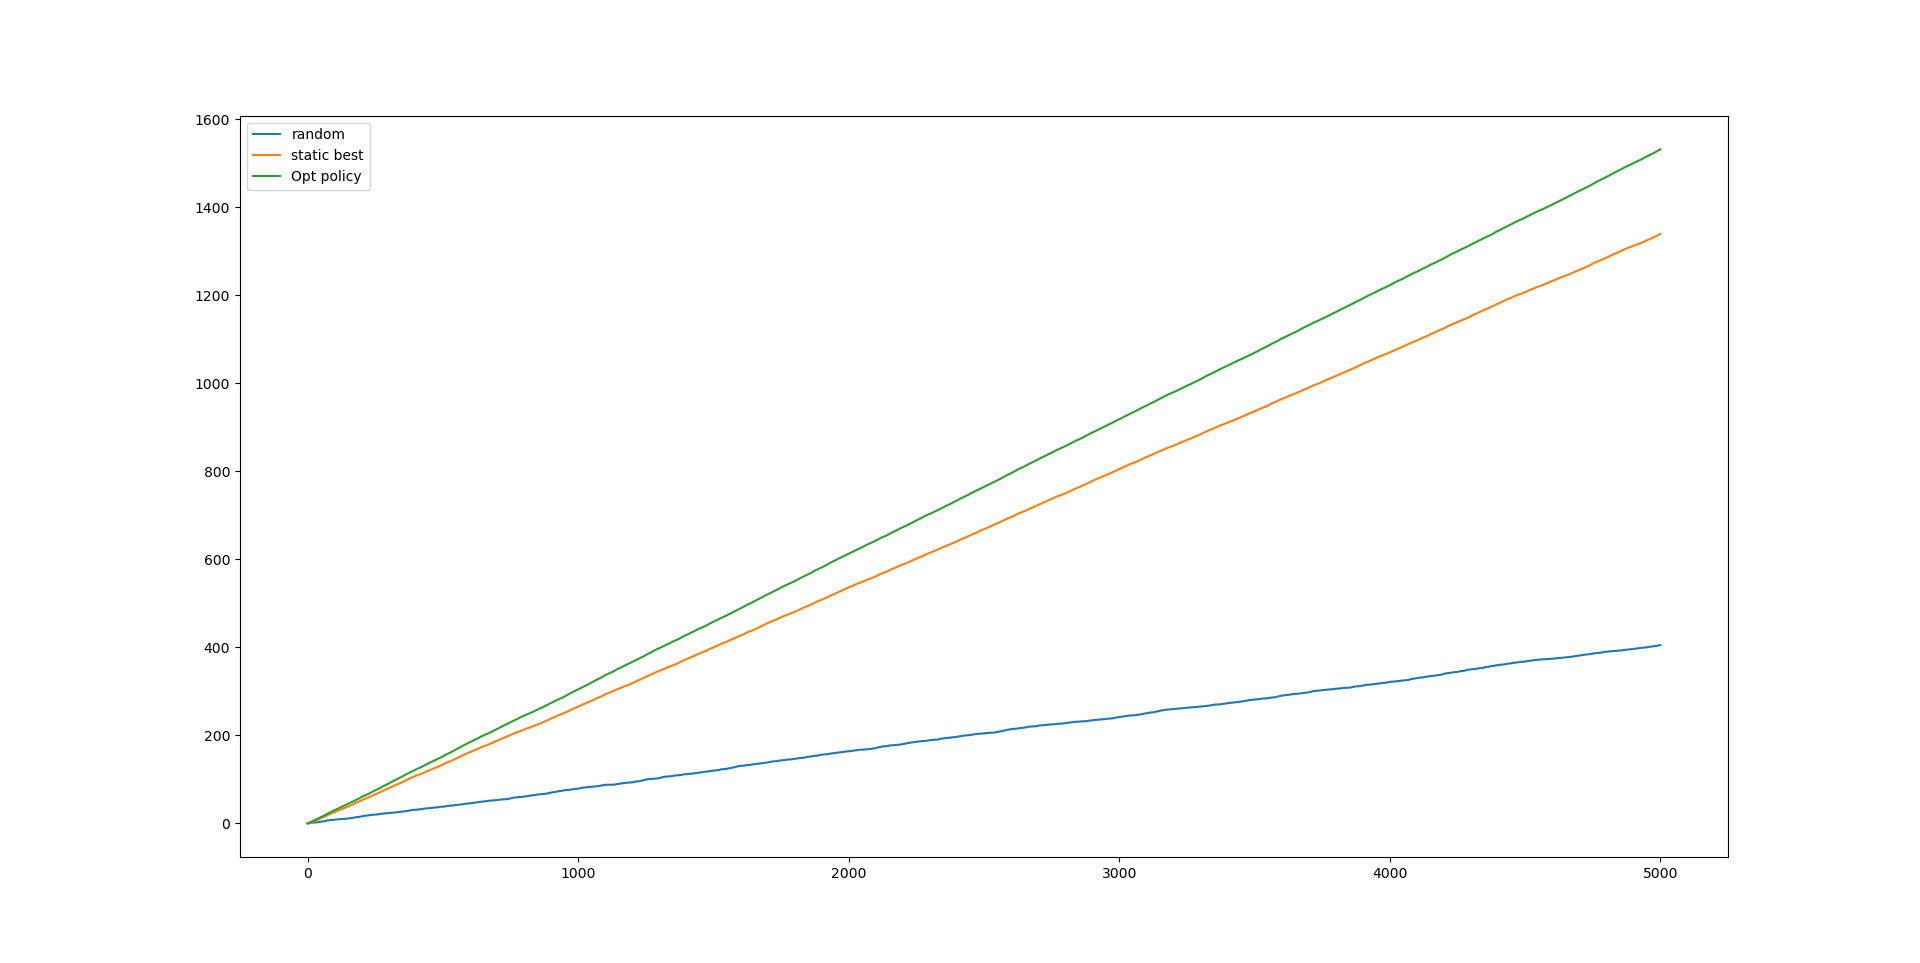
\includegraphics[scale=0.3]{img/baselines.png}
		\caption{Baselines -- agents omniscients}
	\end{figure}
	
	\section{UCB}
	
	\begin{minted}{python}
def upper_bound(t, N, mu):
	"""
	Computes the upper bound of the confidence interval of mean mu
	"""
	return mu + np.sqrt(2 * np.log(t) / N)

def ucb_policy(click_rates):
	"""
	Return the trajectory followed by the agent using ucb policy.
	"""
	
	# Cumulative reward got by each actions
	histo = np.array([click_rates[i][i] for i in range(10)])
	
	# Number of times we took each action
	counter = [1 for i in range(10)]

	# List of the taken action
	action_list = [i for i in range(10)]

	for t in range(10, 5000):
		action = np.argmax([upper_bound(t, counter[i], histo[i] / counter[i]) 
			for i in range(10)])
		counter[action] += 1
		histo[action] += click_rates[t][action]

		action_list.append(action)
	return action_list
	\end{minted}
	
		\begin{figure}[H]
		\centering
		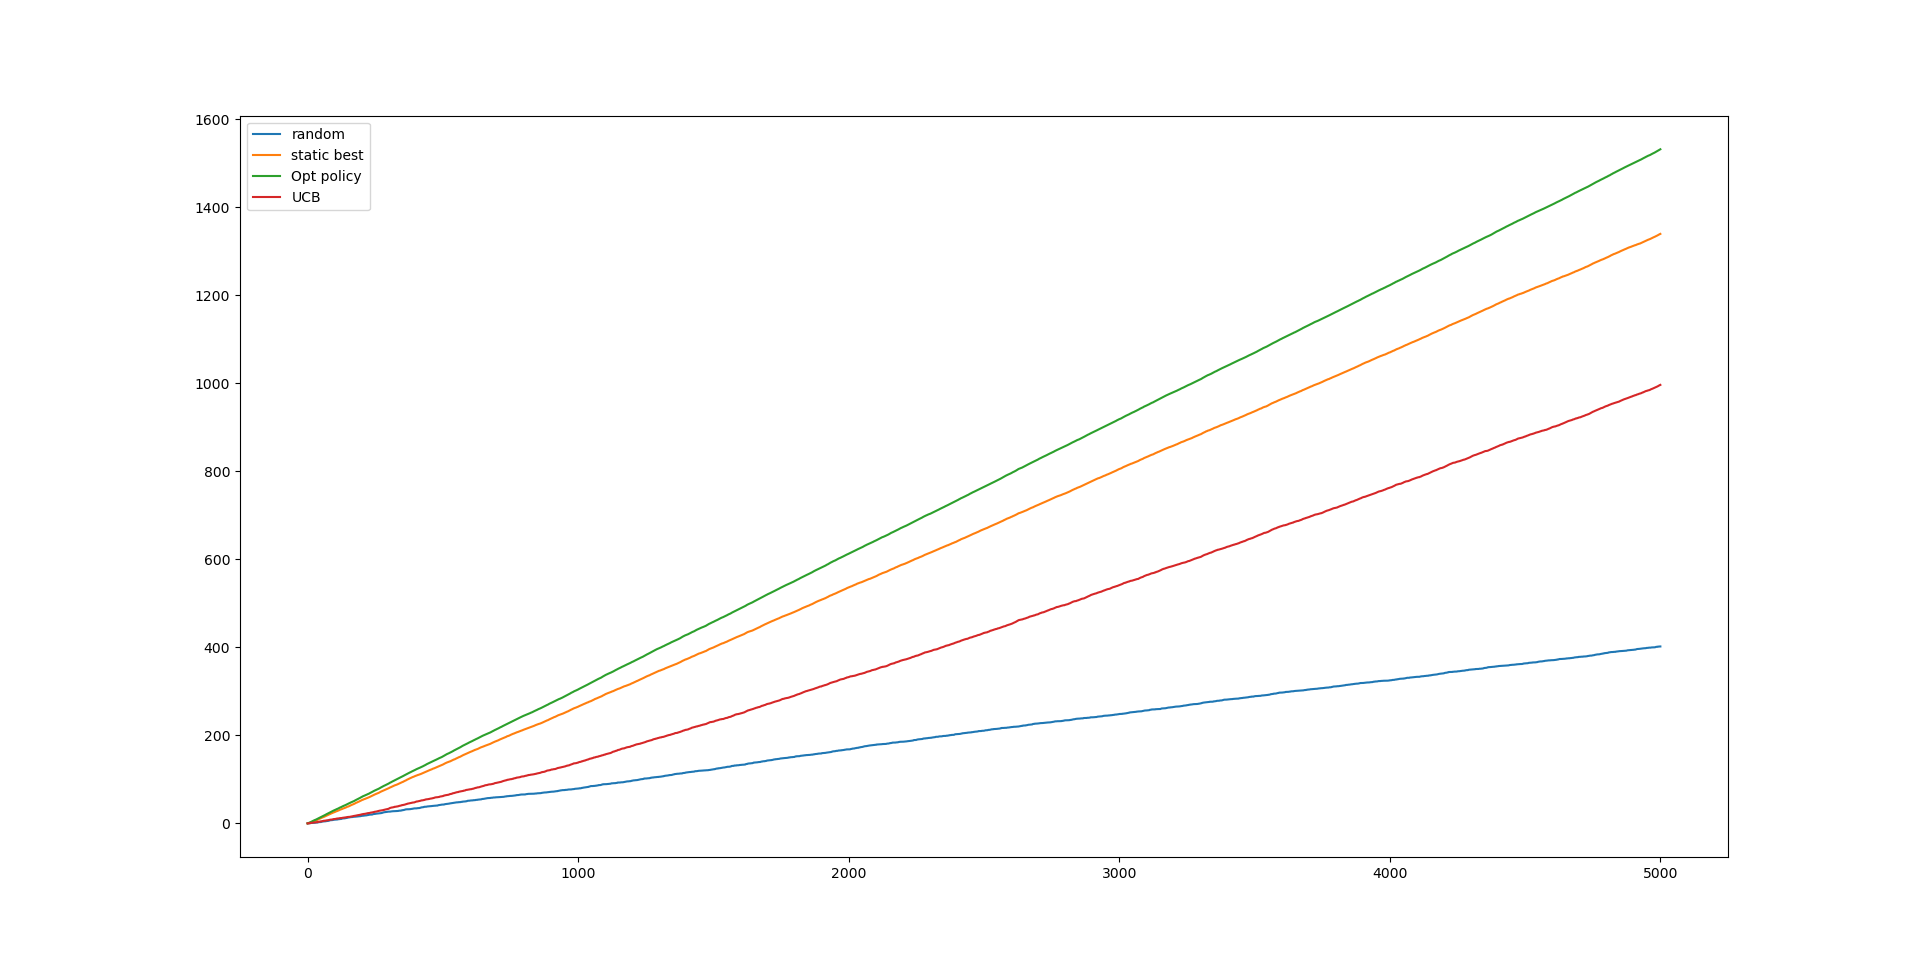
\includegraphics[scale=0.3]{img/ucb.png}
		\caption{Algorithme UCB VS Baselines}
	\end{figure}
	
	\section{LinUCB}
	
	\begin{minted}{python}
def linucb_policy(alpha, articles, click_rates):
	A = [np.identity(5, dtype=float) for i in range(10)]
	b = [np.zeros((5, 1), dtype=float) for i in range(10)]

	theta = [None for i in range(10)]
	pt = [None for i in range(10)]

	actions_list = []

	for t in range(0, 5000):
		for i in range(10):
			theta[i] = np.dot(np.linalg.inv(A[i]), b[i])

			pt[i] = (np.dot(np.transpose(theta[i]),  articles[t]) + alpha * np.sqrt(
			np.dot(
				np.dot(np.transpose(articles[t]),
						np.linalg.inv(A[i])),
				articles[t])))[0]

		at = np.argmax(pt)
		rt = click_rates[t][at]

		A[at] = A[at] + np.dot(np.transpose(articles[t]), articles[t])
		b[at] = b[at] + rt * articles[t]

		actions_list.append(at)

	return actions_list
	\end{minted}
	
	Dans figure suivante on compare \emph{Lin UCB} aux \emph{baselines} en faisant varier $\alpha$. En particulier on vérifie bien qu'un $\alpha$ bas correspond à une forte exploration (ici $\alpha = 0.01$ donne des résultats proches de l'aléatoire) tandis que des valeurs plus importantes permettent un meilleur compromis exploration-exploitation.
	
	\begin{figure}[H]

			\centering
			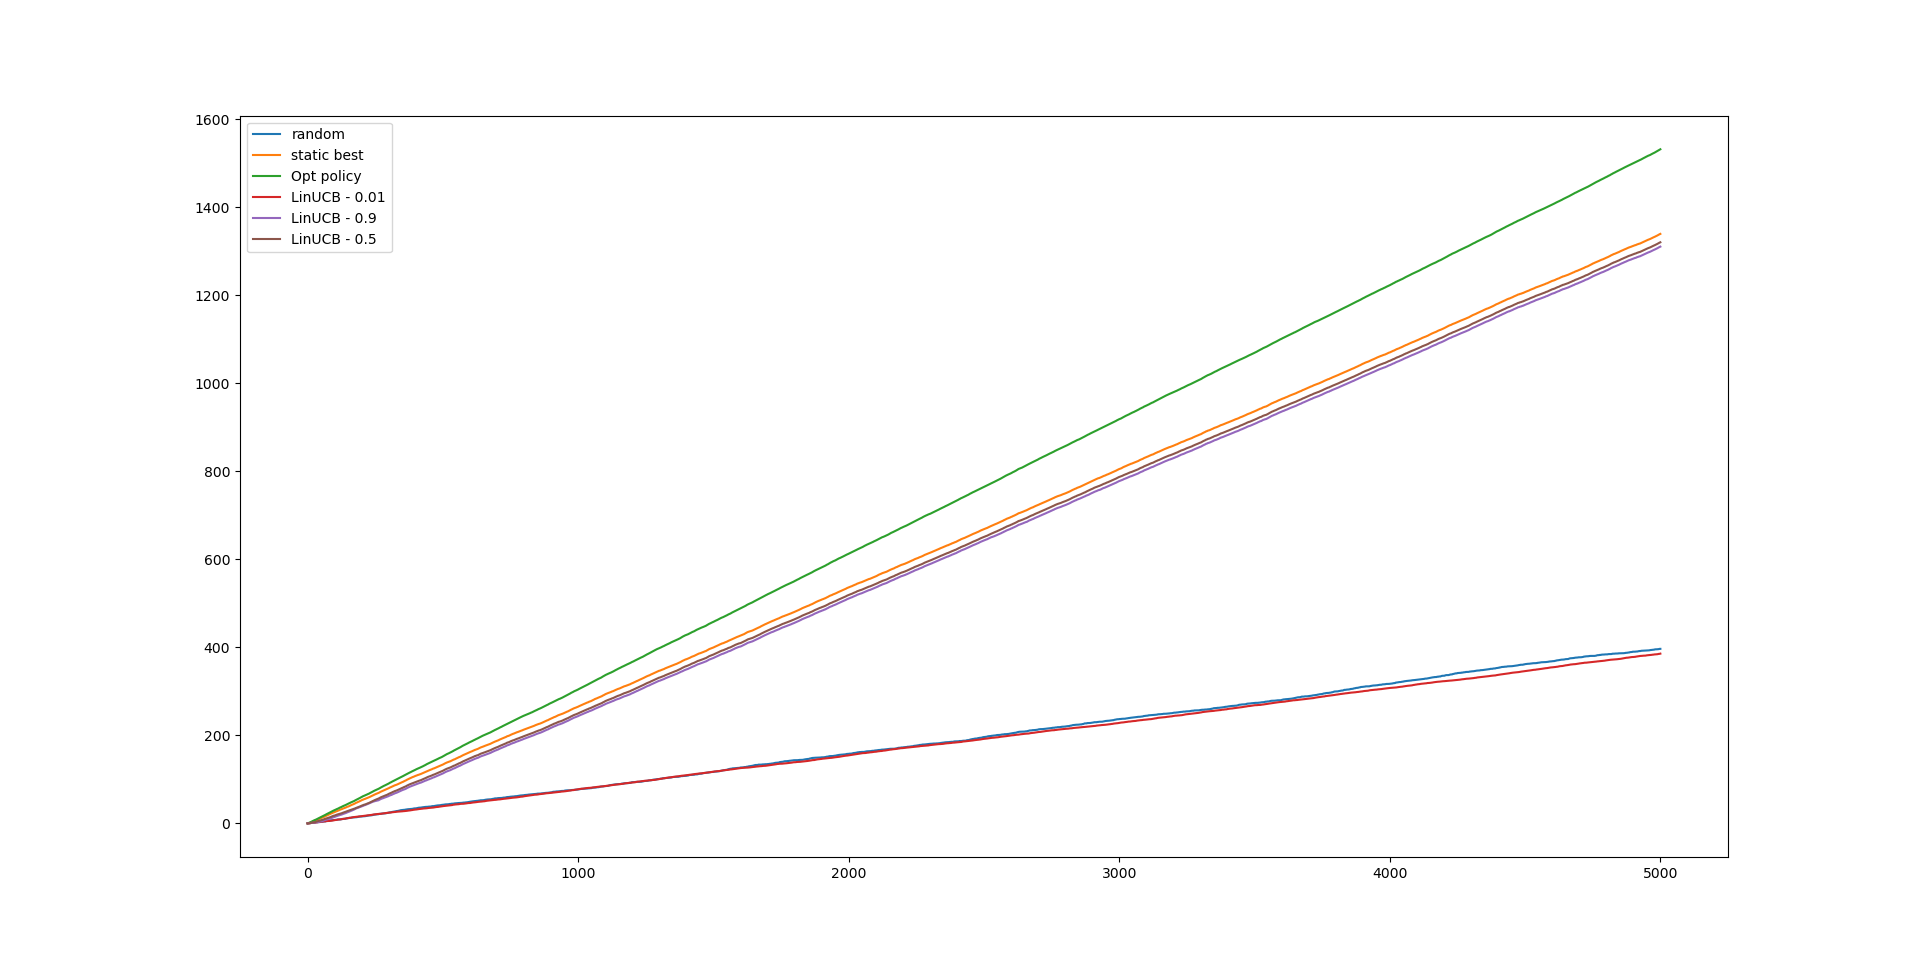
\includegraphics[scale=0.3]{img/lin_ucb.png}
			\caption{Algorithme LinUCB VS Baselines}

	\end{figure}

Par ailleurs, on observe bien que \emph{lin UCB} est clairement meilleur que \emph{UCB}. En effet, en utilisant le contexte pour prendre des décisions plus averties. 

\begin{figure}[H]
	\centering
	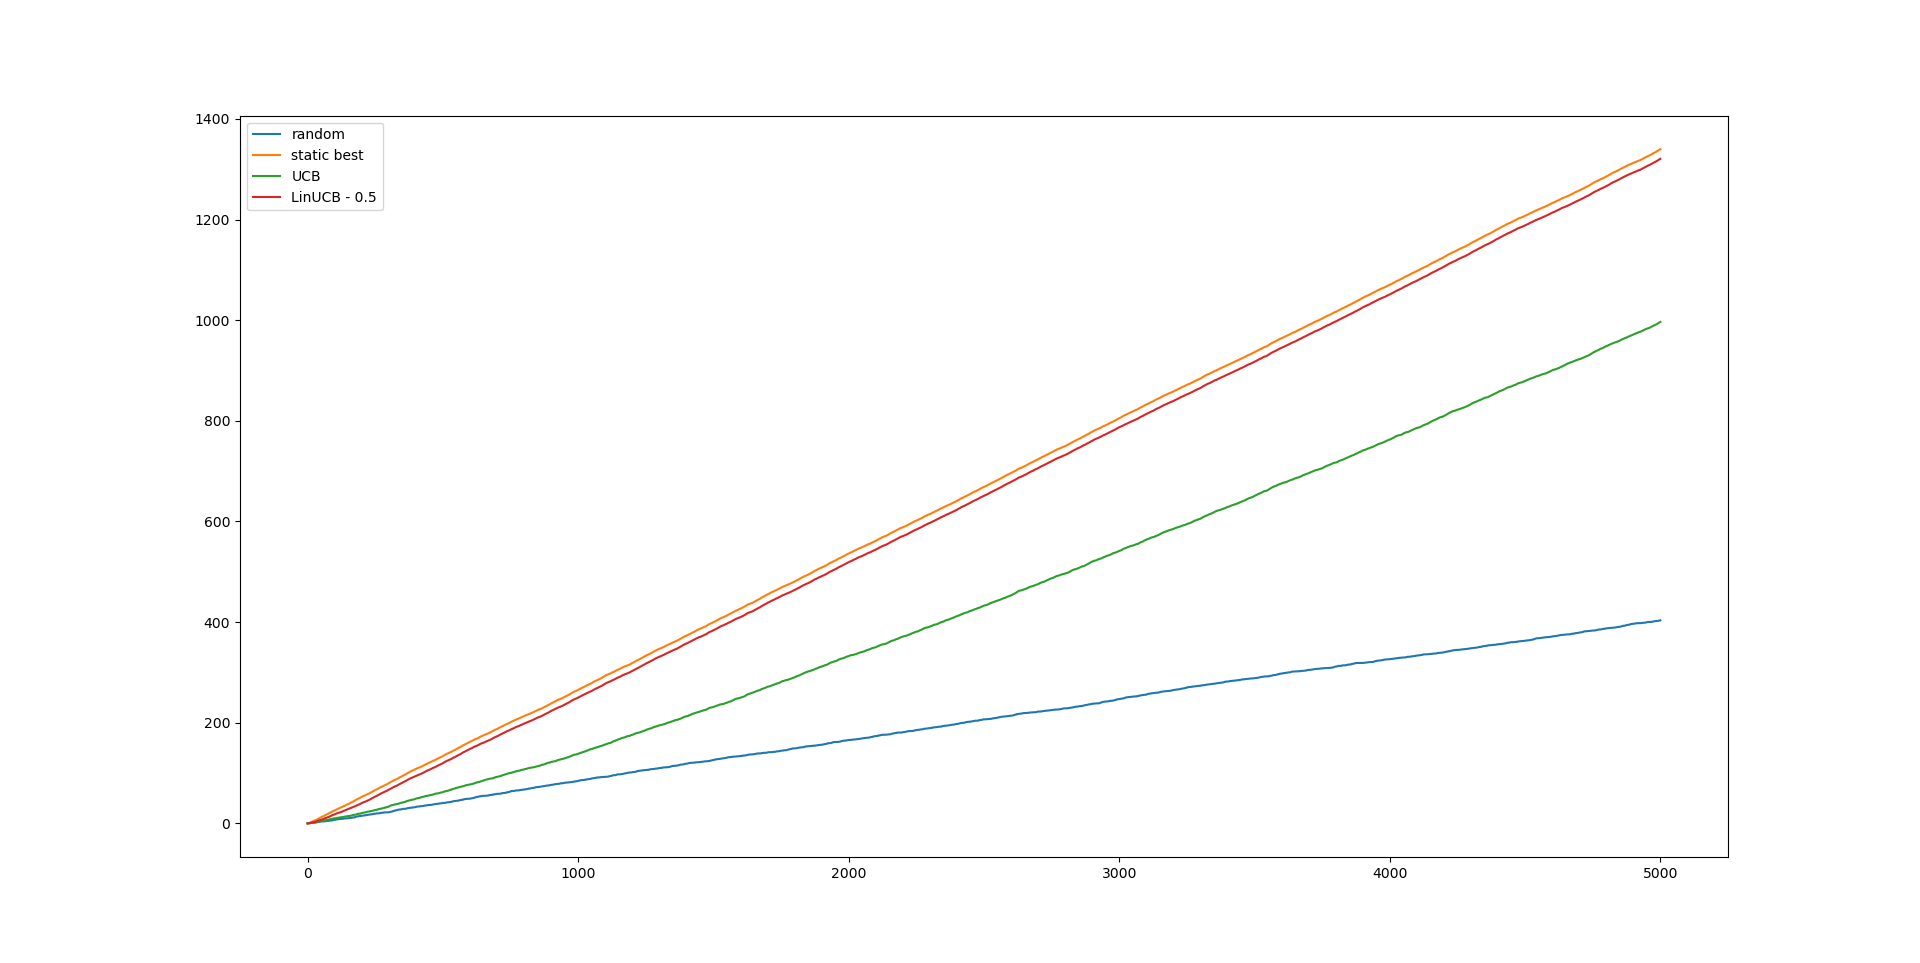
\includegraphics[scale=0.3]{img/linucb_ucb.png}
	\caption{Algorithme LinUCB VS UCB}
\end{figure}


	
	
\end{document}
